\chapter{Adapting a Model Instance Type to Dresden OCL}
\label{chapter:modelInstanceTypeAdaptation}

\begin{flushright}
\textit{Chapter written by Claas Wilke}
\end{flushright}

As mentioned in Chapter~\ref{chapter:architecture}, Dresden OCL is able to
interpret OCL constraints on different types of model instances (e.g., the same
constraints can be interpreted on Java \code{Object}s, \acs{EMF}
\code{EObject}s and \acs{XML} files). This is possible because Dresden OCL
abstracts the instance's elements as \code{IModelInstanceElements}. Thus, each
type of model instance that shall be connected with the OCL Interpreter requires
its own Model Instance Type Adaptation. How such an adaptation has to be
implemented is explained below. First, the different elements that can belong
to a model instance type are presented. Afterwards, the
\code{IModelInstanceProvider}, \code{IModelInstance} and
\code{IModelInstanceFactory} interfaces are explained.


\section{The different types of Model Instance Elements}

Similar to a model, a model instance can have different types of elements. The
element types are similar to the different types that can be expressed in 
models adapted to Dresden OCL.
Figure~\ref{pic:modelInstanceTypeAdaptation:typeHierarchy} shows all different 
types of \code{IModelInstanceElement}s that can exist. The different types are
explained in the following.

\begin{sidewaysfigure}
	\centering
	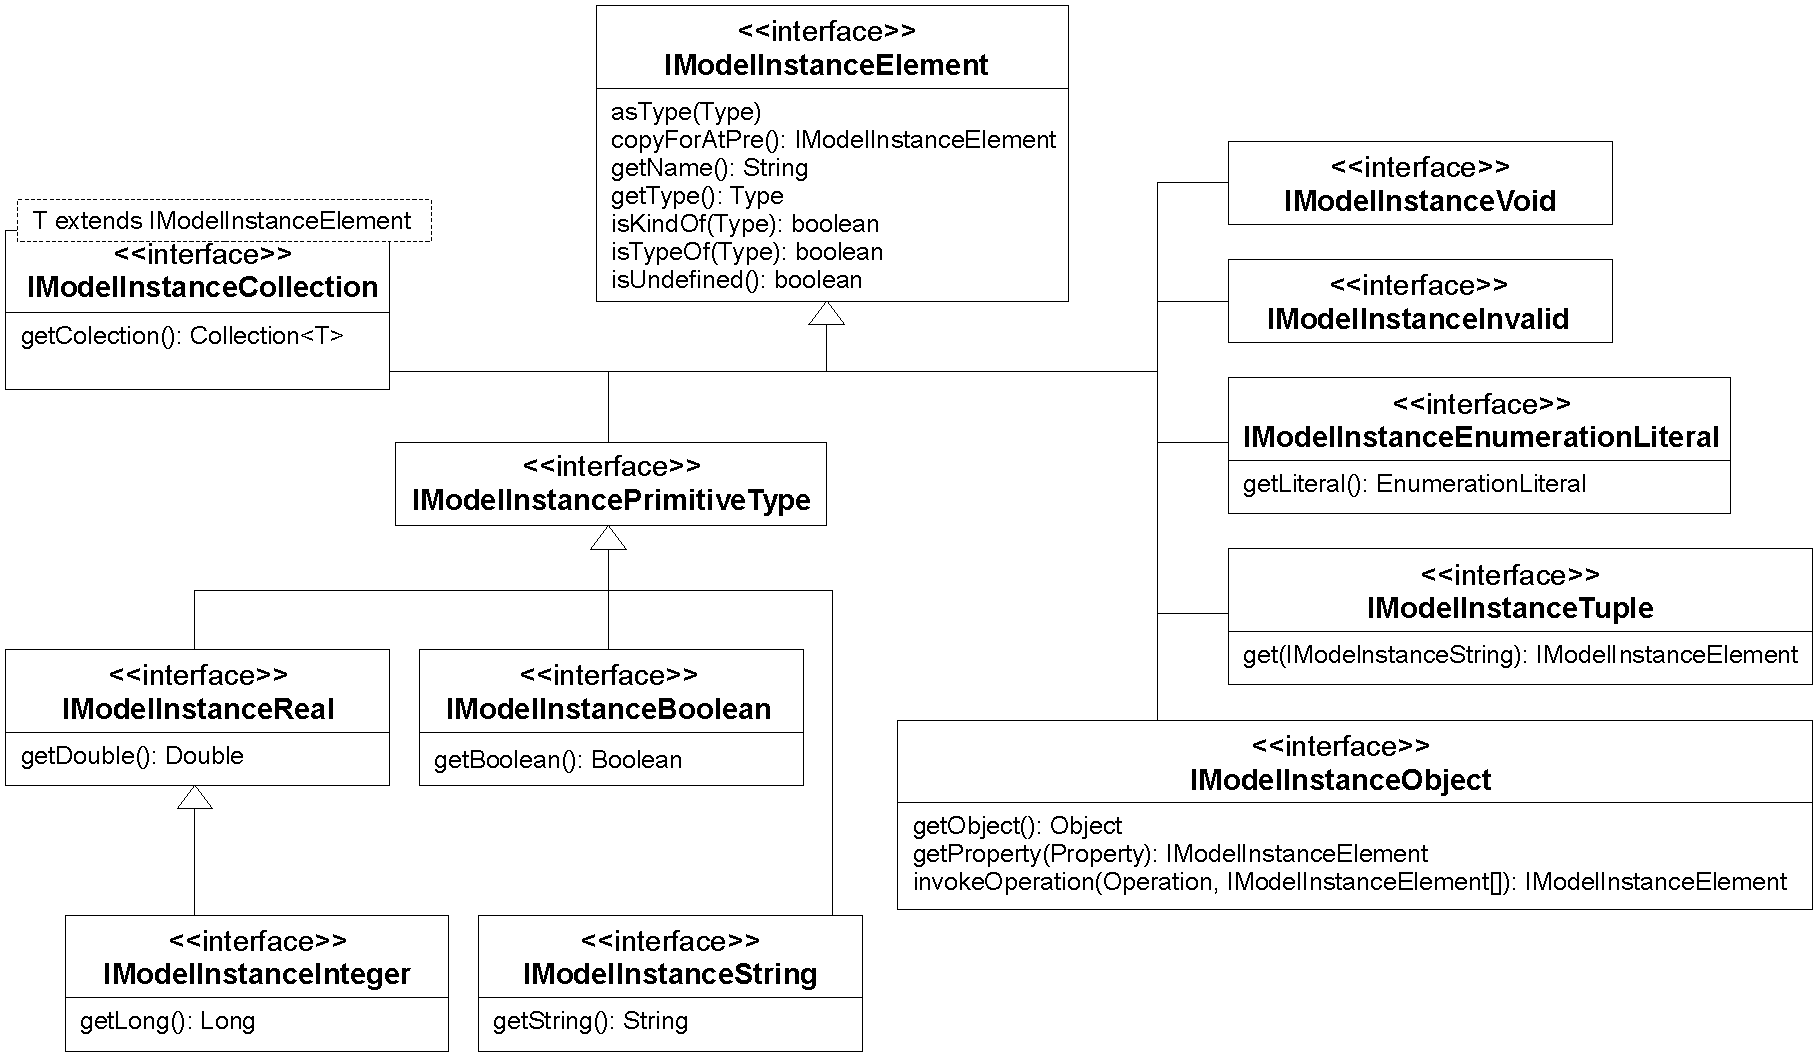
\includegraphics[width=1.0\linewidth]{figures/modelInstanceTypeAdaptation/typeHierarchy}
	\caption{The different types of IModelInstanceElements.}
	\label{pic:modelInstanceTypeAdaptation:typeHierarchy}
\end{sidewaysfigure}


\subsection{The IModelInstanceElement Interface}

Each \code{IModelInstanceElement} has to provide a set of methods that is
required to handle the adapted objects during interpretation. The methods are
shortly explained in the following. Some of these methods are implemented in an
abstract \code{IModelInstanceElement} implementation and have not to be
implemented by every adapter. Nevertheless, they are presented for completeness
reasons.

\subsubsection{asType(Type)}

The method \code{asType(Type)} is required to cast an element to a given type
of its model (e.g., in OCL the primitive type \code{Integer} can be casted to
\code{Real}). In general, this method should check if the given Type conforms
to the adapted element and if so, the result is a new
\code{IModelInstanceElement} of the given type. Else an
\code{AsTypeCastException} is thrown.

\subsubsection{copyForAtPre()} 

The method \code{copyForAtPre()} is required to create a copy of the element if 
its value shall be stored during interpretation as an \keyword{@pre-value}
(e.g., during the interpretation of the constraint

\code{context Person::birthdayHappens()\\
post: self.age = self.age@pre + 1}

the interpreter has to store the value of the property \code{age}). The value
has to be copied, because if \code{age} is incremented during the method's
execution, a simple reference would refer to the incremented
value.\footnote{This is true although age is a primitive type. The integer
instance is modeled in Java and thus can be referenced.} As far as we know, it 
is rather complicate to copy some objects at runtime (e.g., in Java where the 
\code{clone()} method is not visible for every class). Thus, a 
\code{CopyForAtPreException} can be thrown, if an element cannot be copied.

\subsubsection{getName()}

The method \code{getName()} returns a string representation of the element. 
This additional operation exists to provide a different string to display the
element in the GUI components besides the general \code{toString()} method's
result.

\subsubsection{getType()}

The method \code{getType()} returns the implemented \code{Type} of the element.

\subsubsection{isKindOf(Type) and isTypeOf(Type)}

The methods \code{isKindof(Type)} and \code{isTypeOf(Type)} are required to
check if an \code{IModel\-In\-stance\-Ele\-ment} conforms to a given type or is 
of a given type, respectively.

\subsubsection{isUndefined()}

The method \code{isUndefined()} checks if an \code{IModelInstanceElement}'s
adapted element is \code{null} or not.


\subsection{The Adaptation of Model Instance Objects}

The most important \code{IModelInstanceElement} is
the \code{IModelInstanceObject}. It encapsulates the standard objects of a model
instance such as a Java \code{Object} or an \acs{EMF} Ecore \code{EObject}. An
\code{IModelInstanceObject} implementation must be provided by every model
instance type because without this kind of element a model implementation type
does not do any sense. Besides the inherited methods of
\code{IModelInstanceElement} three additional methods have to be implemented.
They are explained below.
 
\subsubsection{getObject()}

The method \code{getObject()} returns the adapted \code{Object} of the 
\code{IModelInstanceObject}.

\subsubsection{getProperty(Property)}

The method \code{getProperty(Property)} is required to get the properties'
values of an object during the interpretation of OCL constraints. The method
should return the adapted value of the given property (probably an
\code{IModelInstanceCollection} of values if the property is of a collection
type or the instance of \code{IModelInstanceVoid} if the property's value is
\code{null}) or throws a \code{Pro\-per\-ty\-Not\-Found\-Ex\-ception} if the
given property does not exist. A \code{PropertyAccessException} can be thrown,
if an unexpected exception occurs during accessing the object's property's
value.

\subsubsection{invokeOperation(Operation, List<IModelInstanceElement>)}
			
The method \code{invokeOperation(Operation, List<IModelInstanceElement>)} is 
required to invoke the adapted object's operations during interpretation. The 
list of arguments (adapted as \code{IModelInstanceElement}s) may be empty but
not \code{null}. The method should return the adapted value of the operation's 
invocation (probably an \code{IModelInstanceCollection} of values if the 
operation is of a collection type or the instance of \code{IModelInstanceVoid}
if the result is \code{null}) or throws an \code{OperationNotFoundException} if
the given operation does not exist. An \code{Operation\-Access\-Ex\-ception}
can be thrown, if an unexpected exception occurs during invoking the object's
operation. This operation is one of the most complicated operations in the 
complete model instance implementation because it must be able to reconvert 
adapted model instance elements given as parameters (e.g., a given 
\code{IModelInstanceObject} has to be unwrapped by calling its 
\code{getObject()} method). For primitive and collection type implementation 
instances this is more complicate because they do not contain an adapted object 
that can be returned. They have to be converted. For details of such a reconvert
mechanism investigate the Java implementation that uses \keyword{Java 
Reflections} to check, whether an operation requires an \code{int}, 
\code{Integer}, \code{byte}, or \code{Long} (for example) as input.


\subsection{The Adaptation of Primitive Type Instances}

To adapt primitive type instances, the interfaces \code{IModelInstanceBoolean}, 
\code{IModel\-In\-stance\-In\-te\-ger}, \code{IModelInstanceReal} and 
\code{IModelInstanceString} exist. Each of them contains an additional method 
to return the adapted value as a Java Object.\footnote{Precisely, a 
\code{Boolean}, a \code{Long}, a \code{Double} or a \code{String}.} Because 
primitive instances do not have any state, they do not have to but can be
implemented by a model instance type. Instead of implementing own primitive 
type instances, the predefined instances \code{JavaModelInstanceBoolean}, 
\code{JavaModelInstanceInteger}, \code{JavaModelInstanceReal} and 
\code{JavaModelInstanceString} (located in the plug-in 
\code{org.dresdenocl.modelinstance} can be reused.


\subsection{The Adaptation of Collections}

Besides primitive type instances and objects, a collection implementation is 
required to describe sets of \code{IModelInstanceElements}. The interface 
\code{IModelInstanceCollection<T extends IModelInstanceElement>} provides three
additional methods explained below. The \code{IModel\-In\-stance\-Col\-lection} 
must not be implemented by every model instance type, the predefined
implementation \code{JavaModelInstanceCollection} can be reused instead.

\subsubsection{getCollection()}

The method \code{getCollection()} returns a Java collection containing the 
\code{IModelInstanceElment}s that are contained in the
\code{IModelInstanceCollection}.


\subsection{IModelInstanceEnumerationLiteral}

The interface \code{IModelInstanceEnumerationLiteral} represents instances of 
\code{Enumerations}. Because enumerations do not have any state, they do not
need any adapted \code{Object}. Thus, a standard 
\code{ModelInstanceEnumerationLiteral} implementation located in the plug-in
\code{org.dresdenocl.\linebreak[0]modelinstance} can be reused. During
adaptation, an enumeration literal existing in the model instance just has to
be associated to its related \code{EnumerationLiteral} in the instance's model.
For details investigate the existing \code{IModelInstance} implementations for 
Java, \acs{EMF} Ecore and \acs{XML}.


\subsection{IModelInstanceTuple}

The interface \code{IModelInstanceTuple} represents key
(\code{IModelInstanceString}) value (\code{IModel\-In\-stance\-Ele\-ment}) data
structures called \keyword{Tuples}. Tuples are required during OCL
interpretation only and cannot be part of a model instance. Thus, a standard
\code{ModelInstanceTuple} implementation located in the plug-in
\code{org.dresdenocl.\linebreak[0]modelinstance} exists.


\subsection{IModelInstanceVoid and IModelInstanceInvalid}

The interfaces \code{IModelInstanceVoid} and \code{IModelInstanceInvalid} exist 
to define the singleton instances of the types \code{OclVoid} and 
\code{OclInvalid}. Their instances can be accessed via the static property 
\code{IModelInstanceVoid.INSTANCE} or \code{IModelInstanceInvalid.INSTANCE}, 
respectively (for example, the \code{IModelInstanceVoid} instance is required
when a method's invocation shall return a \code{null} value).



\section{The IModelInstanceProvider Interface}

Besides the \code{IModelInstaceElements}, a model instance type has to 
implement an \code{IModel\-In\-stance\-Pro\-vider} that has to be registered at 
the model-bus plug-in via the extension point \code{model\-instancetypes}. The 
model instance provider provides the methods to load a resource (given as a 
\code{URL} or \code{File}) into an \code{IModelInstance} object. You can use
the abstract implementation \code{AbstractModelInstanceProvider} to implement
your model instance provider. The two remaining methods to be implemented are 
explained below.


\subsection{getModelInstance(URL, IModel)}

The method \code{getModelInstance(URL, IModel)} is responsible to load a given 
model instance (as a \code{URL}) as an instance of a given model. For 
implementation details investigate the existing implementations for Java, 
\acs{EMF} Ecore and \acs{XML}.


\subsection{createEmptyModelInstance(IModel)}

The method \code{createEmptyModelInstance(IModel)} can be used to create an
empty model instance for a given model. The model instance can be enriched with 
objects during runtime via the method 
\code{IModelInstance.addModelInstanceElement(Object)}.



\section{The IModelInstance Interface}

\begin{figure}
	\centering
	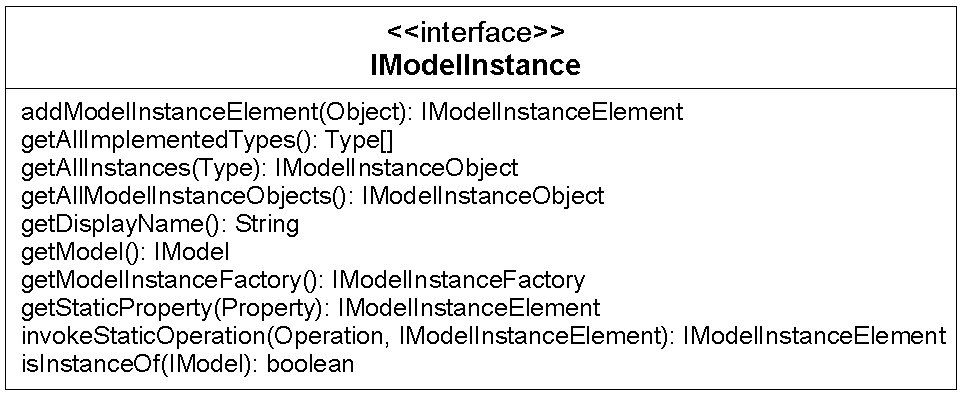
\includegraphics[width=0.8\linewidth]{figures/modelInstanceTypeAdaptation/modelInstanceInterface}
	\caption{The IModelInstance Interface.}
	\label{pic:modelInstanceTypeAdaptation:modelInstanceInterface}
\end{figure}

Figure \ref{pic:modelInstanceTypeAdaptation:modelInstanceInterface} shows the 
interface \code{IModelInstance}. Many of its operations are implemented in the 
abstract basis implementation \code{AbstractModelInstance}. The remaining 
operations that must be implemented are explained below.


\subsection{The Constructor}

The most important operation of a model instance is the constructor. Inside the 
constructor the resource given to the \code{IModelInstanceProvider} is opened
and adapted to \code{IModel\-In\-stance\-Ele\-ments}. To adapt the elements, an 
\code{IModelInstanceFactory} (explained below) is used. For details investigate
the existing \code{IModelInstance} implementations for Java and \acs{EMF}
Ecore.


\subsection{addModelInstanceElement(IModelInstanceElement)}
\label{sect:modelInstanceTypeAdaptation:addIMIElement}

The method \code{addModelInstanceElement(IModelInstanceElement)} can be used to 
add another \code{Object} to the model instance during runtime. The
implementation should use its \code{IModel\-In\-stance\-Fac\-tory} to adapt the 
\code{Object} and throw a \code{TypeNotFoundInModelException} if the given 
\code{Object} can not be adapted to the model instance.


\subsection{getStaticProperty(Property)}

The method \code{getStaticProperty(Property)} is required to get the property 
values of static properties during the interpretation of OCL constraints. The
method should return the adapted value of the static property (probably an
\code{IModelInstanceCollection} of values if the property is of a collection
type or the instance of \code{IModelInstanceVoid} if the property's value is
\code{null}) or throws a \code{PropertyNotFoundException} if the given property
does not exist. A \code{PropertyAccessException} can be thrown, if an unexpected
exception occurs during accessing the object's property.


\subsection{invokeStaticOperation(Operation, List<IModelInstanceElement>)}
			
The method \code{invokeStaticOperation(Operation, List<IModelInstanceElement>)}
is required to invoke static operations during interpretation. The list of 
arguments (adapted as \code{IModel\-In\-stance\-Ele\-ment}s) may be empty but
not \code{null}. The method should return the adapted value of the operation's 
invocation (probably an \code{IModelInstanceCollection} of values if the 
operation is of a collection type or the instance of \code{IModelInstanceVoid}
if the result is \code{null}) or throws an 
\code{Operation\-Not\-Found\-Ex\-ception} if the given operation does not 
exist. An \code{O\-pe\-ra\-tion\-Ac\-cess\-Ex\-cep\-tion} can be thrown, if an
unexpected exception occurs during invoking the object's operation. This
operation is one of the most complicated operations in the complete model
instance implementation because it must be able to reconvert adapted model
instance elements given as parameters (e.g., a given
\code{IModelInstanceObject} can be unwrapped by invoking its \code{getObject()}
method). For primitive and collection type implementations this is more
complicate because they do not contain an adapted object that can be simply
returned. They have to be converted. For details of such a reconvert mechanism
investigate the Java implementation that uses \keyword{Java Reflections} to
check, whether an operation requires an \code{int}, \code{Integer},
\code{byte}, or \code{Long} (for example) as input.



\section{The IModelInstanceFactory Interface}

\begin{figure}
	\centering
	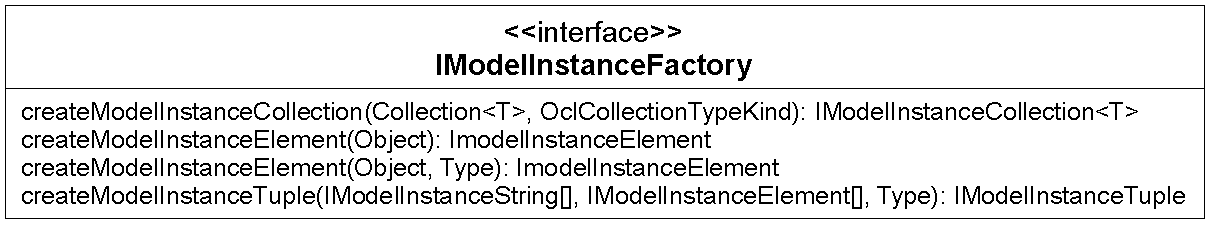
\includegraphics[width=1.0\linewidth]{figures/modelInstanceTypeAdaptation/modelInstanceFactoryInterface}
	\caption{The IModelInstanceFactory Interface.}
	\label{pic:modelInstanceTypeAdaptation:modelInstanceFactoryInterface}
\end{figure}

The \code{IModelInstanceFactory} implementation of a model instance is
responsible to adapt the instance's objects to the \code{IModelInstanceElement} 
implementations. It investigates the types of the objects to decide if they
shall be adapted as \code{IModelInstanceObject}s, 
\code{IModelInstance\-Pri\-mi\-tive\-Type}s or
\code{IModelInstanceEnumerationLiteral}s. An \code{IModelInstanceFactory} has
to implement four methods as shown in 
Figure~\ref{pic:modelInstanceTypeAdaptation:modelInstanceFactoryInterface}. A 
default implementation for the basis elements such as
\code{IModelInstanceTuples} and \code{IModelInstanceCollections} called 
\code{BasisJavaModel\-In\-stance\-Fac\-tory} exists. Normally, an 
\code{IModelInstanceFactory} should extend the 
\code{BasisJava\-Mo\-del\-In\-stance\-Factory} and should call the methods of
the basis implementation as often as possible (e.g., to adapt the 
\code{IModelInstanceTuples}). For details investigate the existing
implementations for \acs{EMF} Ecore, Java and \acs{XML}.



\section{Adapting an own Model Instance Type}

We know that adapting a model instance type sounds easy but can be a lot
of pain. Every kind of model instance comes with its own problems and
solutions. Some may be simple, others may be complicate or impossible. But never
forget, if you adapted your own type of model instance, you can connect your
instances with Dresden OCL and you can reuse the OCL Parser and OCL Interpreter!

If you are confused and still do not know how to adapt your model instance type,
investigate the existing adaptations for Java
(\code{org.dresdenocl.modelinstancetype.java}), \acs{EMF} Ecore
(\code{org.dresdenocl.modelinstancetype.ecore}) and \acs{XML}
(\code{org.dresdenocl.modelinstancetype.\linebreak[0]xml}). To check your
adaptation, have a look at the \keyword{Generic Model Implementation Type Test
Suite} (presented in Chapter~\ref{chapter:modelInstanceTestSuite}) as well.
